\section{Experiment}

\subsection{Setup}
We simulate an honest party network with 37 nodes and adversary network with 12
nodes. This sets the adversary hash rate ($\beta$) for the experiments at 24.44.
PoEM experiments use a bias of 14.6. Our simulations measure the confirmation
delay(d) under different block rates(g) for both PoEM and bitcoin. For each
experiment g value is fixed and is run as a monte carlo simulation with 100
runs. For each run the winner at each round is calculated by looking at which
party reached the round the fastest from the start of the experiment. After
after 100 runs, wins for the honest party is added up for each run and the f is
calculated by picking the expected number of blocks for which the probability of
honest parties winning crosses 90\%. Confirmation delay(d) is calculated by
dividing the f by g for each experiment. Fig1 shows the evolution of d for
different values of g. Best operating conditions for a protocol is the point of
least confirmation delay. Bitcoin achieved the lowest delay of 11.16 for g=0.98
and for PoEM achieved lowest delay of 10.58 for g=1.29. This shows that PoEM can
be run 31.6\% faster rate and still achieve a lower d.

We also ran simulation of PoEM with different bias values at the best operating
point of Bitcoin at g=0.98. Fig2 shows the confirmation delay for different
values of g. It can be seen that PoEM can achieve even lower confirmation delays
for lower values of bias. The best confirmation delay of 7.95 was achieved with
bias of 10.

\begin{figure}
    \centering
    \begin{subfigure}{0.49\textwidth}
    \centering
    \caption{d vs g}
    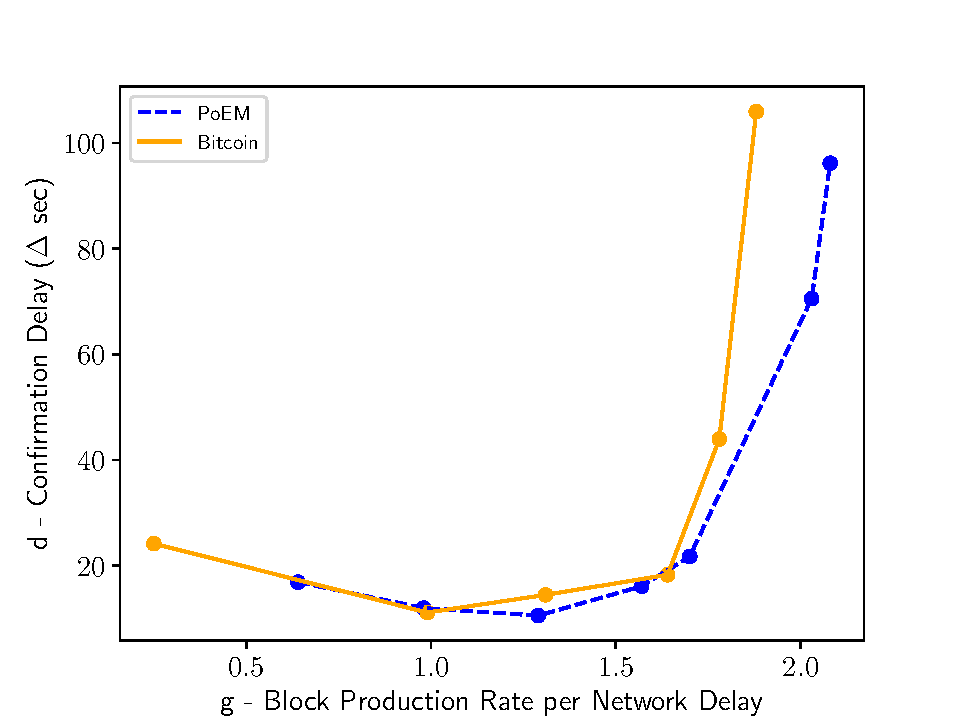
\includegraphics[width = \textwidth]{figures/dvsg.pdf}
    \label{fig:dvsg}
    \end{subfigure}
    \begin{subfigure}{0.49\textwidth}
    \centering
    \caption{d vs bias}
    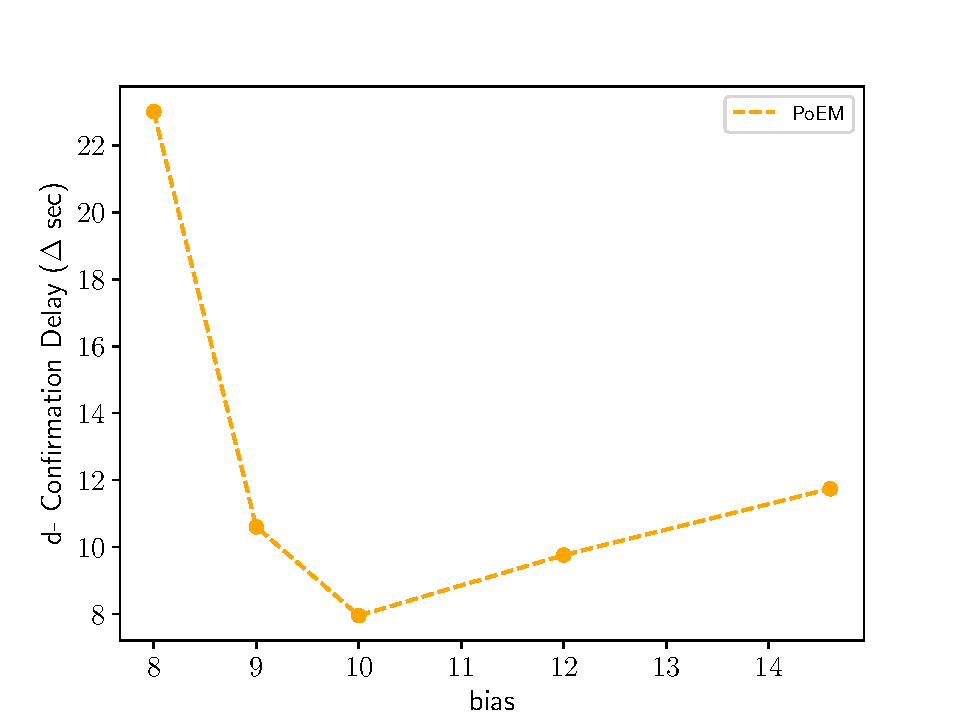
\includegraphics[width = \textwidth]{figures/gamma.pdf}
    \label{fig:right}
    \end{subfigure}
    \caption{description}
    \label{fig:gamma}
\end{figure}

\subsection{Practical Deployment}
PoEM consensus mechanism has been deployed in real world as a consensus
mechanism for the Quai Networks Iron Age Testnet. The testnet was started in
October 2023 and has been running since. As of 24th Jan 2024, over 7.5 million
blocks have been mined with over 2000 Miners, Node operators participating in
the testnet and over 500 million transactions have been confirmed in the network
using the consensus mechanism. The network has maintained an average hash rate
of over 50GH/s during this time period.